\section{Fase 3: Optimización}

Un paso de ETL ejecutado una sola vez por versión reduce el tiempo de análisis entre $10\times$ y $110\times$, y se amortiza antes de completar una sola corrida.

\subsection{Diagnóstico}

De la Fase 2 salen cuatro hechos que definen qué optimizar:

\begin{enumerate}
  \item La carga domina el tiempo total, y como cada pregunta recarga el archivo, ese costo se paga tres veces.
  \item Se leen nueve columnas y solo se usan tres: \texttt{start\_rental\_date\_time}, \texttt{start\_station\_id} y \texttt{end\_station\_id}. Las dos columnas de nombres de estación son las más pesadas y además son redundantes, porque ya están normalizadas en el catálogo.
  \item Los tipos están sobredimensionados. Los identificadores de estación llegan a $\sim$800 y viven en \texttt{INT64} o \texttt{DOUBLE}; la hora y el día se recalculan desde el timestamp en cada consulta.
  \item SQLite recorre filas completas y parsea timestamps con \texttt{strftime} registro por registro.
\end{enumerate}

\subsection{La optimización elegida}

Pre-procesar a un artefacto columnar con tipos reducidos, sobre el cual corren después todas las consultas.

\begin{table}[htbp]
\centering
\footnotesize
\caption{Decisiones de la optimización}
\label{tab:fase3-decisiones}
\begin{tabularx}{\textwidth}{>{\raggedright\arraybackslash}p{4.2cm}X}
\toprule
Decisión & Por qué mejora el rendimiento \\
\midrule
Formato Parquet, para Pandas y DuckDB & Binario y columnar: el motor lee solo las columnas de la consulta y no parsea texto. Trae esquema y tipos embebidos, así que no hay inferencia. \\
CSV estrecho de 4 enteros, para SQLite & SQLite no lee Parquet. Su artefacto es un CSV con cuatro columnas numéricas cortas: el parseo por fila se abarata frente a nueve campos con dos cadenas largas y dos timestamps. \\
Proyección a 4 columnas & Se eliminan \texttt{rental\_id}, \texttt{bike\_id}, \texttt{duration}, los dos nombres y \texttt{end\_rental\_date\_time}. Menos bytes leídos por fila. \\
Pre-cálculo de \texttt{dia\_semana} y \texttt{hora} & Se hace una vez en el ETL en vez de en cada consulta, y se guardan como \texttt{TINYINT}. \\
Tipos reducidos (\texttt{TINYINT}, \texttt{SMALLINT}) & Menos memoria por fila y mejor aprovechamiento de caché. \\
Ordenar por \texttt{dia\_semana, hora} & Potencia la codificación RLE de Parquet y reduce el tamaño en disco. \\
Índice covering por pregunta en SQLite & Cada consulta recibe únicamente el índice que necesita, en vez de construir tres y usar uno. \\
\bottomrule
\end{tabularx}
\end{table}

El artefacto Parquet de la versión XL pesa 89 MB frente a los 4,725 MB del CSV original: una reducción de $53\times$.

\subsection{Impacto medido}

Tiempo total de las tres preguntas, antes y después, en segundos.

\begin{table}[htbp]
\centering
\footnotesize
\caption{Impacto de la optimización por versión y equipo}
\label{tab:fase3-impacto}
\begin{tabularx}{\textwidth}{llXXXr}
\toprule
Versión & Equipo & Pandas & DuckDB & SQLite & ETL (s) \\
\midrule
M  & Pc\_Jesus  & $34.5$ a $0.7$ ($48\times$) & $5.0$ a $0.6$ ($8\times$) & $108.2$ a $61.7$ ($1.8\times$) & 8.4 \\
M  & Pc\_Martha & $50.0$ a $2.5$ ($20\times$) & $6.7$ a $2.0$ ($3\times$) & $164.6$ a $184.4$ ($0.9\times$) & 2.9 \\
M  & Pc\_Nahin  & $143.1$ a $3.9$ ($36\times$) & $15.3$ a $3.8$ ($4\times$) & $445.0$ a $221.7$ ($2.0\times$) & 8.4 \\
L  & Pc\_Jesus  & $79.1$ a $3.2$ ($25\times$) & $11.5$ a $1.0$ ($11\times$) & $232.8$ a $129.4$ ($1.8\times$) & 2.6 \\
L  & Pc\_Martha & $106.5$ a $4.6$ ($23\times$) & $15.3$ a $2.7$ ($6\times$) & $404.0$ a $304.1$ ($1.3\times$) & 5.4 \\
L  & Pc\_Nahin  & $288.1$ a $6.0$ ($48\times$) & $25.9$ a $6.5$ ($4\times$) & $776.9$ a $483.8$ ($1.6\times$) & 5.4 \\
XL & Pc\_Jesus  & $195.4$ a $3.4$ ($57\times$) & $27.3$ a $2.7$ ($10\times$) & $472.6$ a $291.5$ ($1.6\times$) & 6.3 \\
XL & Pc\_Martha & falló a $6.0$ & falló a $3.1$ & falló a $486.0$ & 10.6 \\
XL & Pc\_Nahin  & $501.4$ a $14.4$ ($35\times$) & $122.3$ a $14.6$ ($8\times$) & ver nota \S\ref{sec:nota-nahin} & 14.8 \\
\bottomrule
\end{tabularx}
\end{table}

En Pc\_Jesus, versión XL, las mejoras por pregunta llegan a $110\times$ en Pandas Q2 (57.1 s a 0.52 s).

\subsection{Amortización del ETL}

El ETL se paga una sola vez y el ahorro se cobra en cada corrida posterior. En la versión XL sobre Pc\_Jesus, el ETL cuesta 6.3 s y ahorra 191.9 s por corrida en Pandas: \textbf{se amortiza en el 3\% de una corrida}. En DuckDB, que ya era rápido, el ahorro es de 24.6 s por corrida y la amortización toma el 26\% de una corrida. En un pipeline que se ejecuta a diario la inversión se recupera de inmediato; para un análisis único aislado, el cálculo es menos evidente, y ese contraste es parte del resultado.

\subsection{Nota sobre SQLite en la versión XL de Pc\_Nahin}
\label{sec:nota-nahin}

Una lectura superficial de la gráfica sugiere que la optimización empeoró SQLite en esa máquina: 1,099.2 s en base contra 1,157.8 s optimizado. \textbf{La comparación no es válida.} En la etapa base, Q2 tardó 678.7 s y quedó marcada como \texttt{EXCEDE} por superar los 10 minutos, lo que hizo que el harness omitiera automáticamente Q3. Ese 1,099.2 es la suma de \textbf{dos} preguntas; el 1,157.8 es la suma de \textbf{tres}.

Comparando pregunta contra pregunta:

\begin{table}[htbp]
\centering
\caption{SQLite XL en Pc\_Nahin, comparación pregunta contra pregunta}
\label{tab:nahin-sqlite}
\begin{tabular}{lrrl}
\toprule
Pregunta & Base (s) & Optimizado (s) & Mejora \\
\midrule
Q1 & 420.5 & 237.8 & $1.77\times$ \\
Q2 & 678.7 (EXCEDE) & 539.5 & $1.26\times$ \\
Q3 & no ejecutada & 380.5 & de imposible a viable \\
\bottomrule
\end{tabular}
\end{table}

La optimización no solo ayudó: convirtió una ejecución que violaba el límite del enunciado en una que lo cumple.

\subsection{Por qué SQLite gana menos que las demás}

SQLite es la herramienta más castigada en la línea base y la que más gana en términos absolutos con el esquema estrecho. Pero \textbf{su ingesta sigue siendo proporcional al número de filas}: el \texttt{executemany} tiene que insertar los mismos millones de registros, solo que con campos más baratos de parsear. Por eso su mejora es grande pero no del orden de la de Pandas, y sigue sin alcanzar a DuckDB.

En Pc\_Martha, versión M, la optimización incluso resultó marginalmente más lenta (164.6 s contra 184.4 s). La causa es que construir el índice covering sobre 9.6 millones de filas cuesta más de lo que ahorra el parseo del CSV estrecho en esa máquina. \textbf{Una optimización no es universalmente buena: su valor depende de dónde estaba el cuello de botella.}

\begin{figure}[htbp]
  \centering
  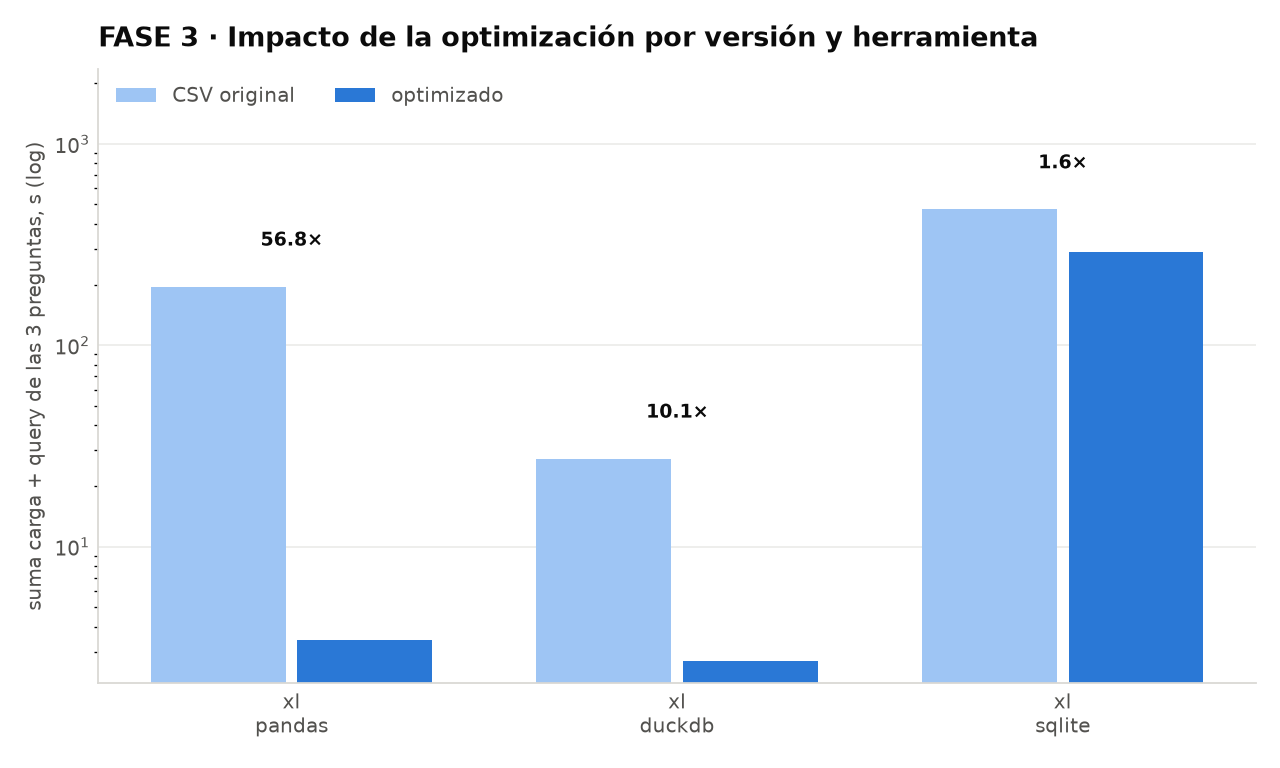
\includegraphics[width=0.75\textwidth]{figuras/fase3_impacto_pc_jesus.png}
  \caption{Impacto de la optimización por herramienta, Pc\_Jesus (base vs. optimizado).}
  \label{fig:fase3-impacto}
\end{figure}
